% RESULTS (~1.5-2 pages). Prompt: AGENT_PROMPTS.md, section "Results".
% Keep the table/figure commands; only describe what the tables show. Numbers must match fact_sheet.md.
\section{Results}
\label{sec:results}

\begin{figure}[t]
\centering
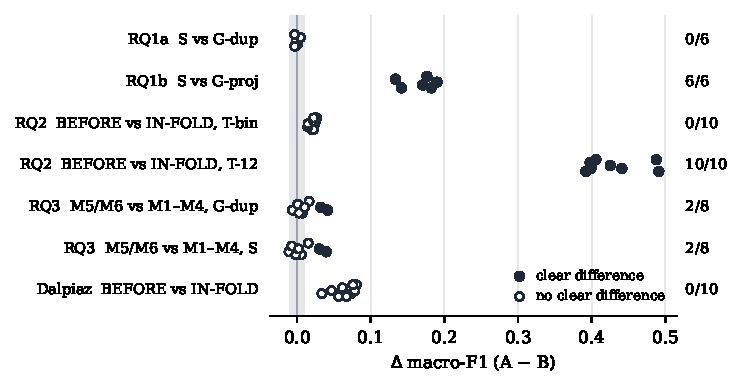
\includegraphics[width=\columnwidth]{figures/summary_deltas.pdf}
\caption{Mean paired difference in macro-F1 for every planned comparison (one dot per model or model$\times$oversampler). Filled: clear difference ($|\Delta| \geq 0.01$ and Holm-adjusted $p < 0.05$); hollow: no clear difference. Grey band: $|\Delta| < 0.01$. Right: clear differences per family.}
\label{fig:summary}
\end{figure}

\subsection{RQ1: Duplicate- and project-grouped evaluation}
\begin{table*}[t]
\centering
\caption{RQ1: macro-F1 under stratified CV (S), duplicate-grouped CV (G-dup) and project-grouped CV (G-proj) on PROMISE\_exp, T-bin, no oversampling. $\Delta$ = S $-$ grouped (difference of means). $\Delta$ is computed from unrounded scores. Descriptive only: the protocols use different test folds, so no paired test is applied (mean $\pm$ SD over 5 seeds $\times$ 5 folds).}
\label{tab:rq1}
\small
\setlength{\tabcolsep}{4pt}
\begin{tabular}{lrrrrr}
\toprule
& \multicolumn{3}{c}{Macro-F1} & \multicolumn{2}{c}{$\Delta$} \\
\cmidrule(lr){2-4}\cmidrule(lr){5-6}
Model & S & G-dup & G-proj & S $-$ G-dup & S $-$ G-proj \\
\midrule
M0 & $0.351 \pm 0.000$ & $0.351 \pm 0.000$ & $0.352 \pm 0.008$ & -- & -- \\
M1 & $0.876 \pm 0.020$ & $0.878 \pm 0.025$ & $0.694 \pm 0.094$ & $-0.002$ & $+0.182$ \\
M2 & $0.893 \pm 0.019$ & $0.891 \pm 0.018$ & $0.722 \pm 0.061$ & $+0.001$ & $+0.171$ \\
M3 & $0.851 \pm 0.031$ & $0.853 \pm 0.022$ & $0.661 \pm 0.113$ & $-0.001$ & $+0.190$ \\
M4 & $0.889 \pm 0.019$ & $0.884 \pm 0.025$ & $0.755 \pm 0.055$ & $+0.005$ & $+0.134$ \\
M5 & $0.882 \pm 0.023$ & $0.885 \pm 0.019$ & $0.705 \pm 0.083$ & $-0.003$ & $+0.176$ \\
M6 & $0.891 \pm 0.018$ & $0.894 \pm 0.019$ & $0.749 \pm 0.052$ & $-0.003$ & $+0.142$ \\
\bottomrule
\end{tabular}
\end{table*}

TODO: RQ1 text.

\subsection{RQ2: Oversampling before vs.\ inside the training fold}
\begin{table*}[t]
\centering
\caption{RQ2: macro-F1 when oversampling is applied to the whole dataset before splitting (BEFORE) versus inside each training fold only (IN-FOLD), PROMISE\_exp, stratified CV. OS-R: random oversampling; OS-S: SMOTE. $\Delta$ = BEFORE $-$ IN-FOLD. Bold $\Delta$: clear difference ($|\Delta| \geq 0.01$ and Holm-adjusted $p < 0.05$, corrected repeated k-fold $t$-test).}
\label{tab:rq2}
\small
\setlength{\tabcolsep}{4pt}
\begin{tabular}{ll cc rr cc rr}
\toprule
& & \multicolumn{4}{c}{T-bin (FR vs NFR)} & \multicolumn{4}{c}{T-12 (12 classes)} \\
\cmidrule(lr){3-6}\cmidrule(lr){7-10}
Model & OS & BEFORE & IN-FOLD & $\Delta$ & $p_{\mathrm{Holm}}$ & BEFORE & IN-FOLD & $\Delta$ & $p_{\mathrm{Holm}}$ \\
\midrule
M1 & OS-R & 0.899 & 0.878 & +0.020 & 0.687 & 0.989 & 0.597 & \textbf{+0.392} & $<$0.001 \\
M1 & OS-S & 0.900 & 0.879 & +0.021 & 0.712 & 0.988 & 0.589 & \textbf{+0.399} & $<$0.001 \\
M2 & OS-R & 0.917 & 0.893 & +0.024 & 0.687 & 0.992 & 0.593 & \textbf{+0.399} & $<$0.001 \\
M2 & OS-S & 0.920 & 0.894 & +0.026 & 0.194 & 0.992 & 0.595 & \textbf{+0.398} & $<$0.001 \\
M3 & OS-R & 0.882 & 0.855 & +0.027 & 0.621 & 0.994 & 0.506 & \textbf{+0.488} & $<$0.001 \\
M3 & OS-S & 0.878 & 0.855 & +0.023 & 0.712 & 0.986 & 0.495 & \textbf{+0.491} & $<$0.001 \\
M4 & OS-R & 0.903 & 0.888 & +0.015 & 0.712 & 0.967 & 0.526 & \textbf{+0.441} & $<$0.001 \\
M4 & OS-S & 0.905 & 0.890 & +0.015 & 0.712 & 0.951 & 0.525 & \textbf{+0.425} & $<$0.001 \\
M5 & OS-R & 0.909 & 0.886 & +0.023 & 0.712 & 0.992 & 0.595 & \textbf{+0.398} & $<$0.001 \\
M5 & OS-S & 0.908 & 0.885 & +0.023 & 0.687 & 0.993 & 0.587 & \textbf{+0.406} & $<$0.001 \\
\bottomrule
\end{tabular}
\end{table*}

TODO: RQ2 text.

\subsection{RQ3: Ensembles under leakage-aware evaluation}
\begin{table}[t]
\centering
\caption{RQ3: ensembles (M5 hard voting, M6 stacking) versus single classifiers M1--M4, PROMISE\_exp, T-bin, macro-F1. $\Delta$ = ensemble $-$ single; 95\% CI from the corrected $t$-test (unadjusted). G-dup is the primary protocol; S is reported for comparison. Bold $\Delta$: clear difference ($|\Delta| \geq 0.01$ and Holm-adjusted $p < 0.05$, corrected repeated k-fold $t$-test).}
\label{tab:rq3}
\small
\setlength{\tabcolsep}{4pt}
\begin{tabular}{l rcr rr}
\toprule
& \multicolumn{3}{c}{G-dup (primary)} & \multicolumn{2}{c}{S} \\
\cmidrule(lr){2-4}\cmidrule(lr){5-6}
Comparison & $\Delta$ & 95\% CI & $p_{\mathrm{Holm}}$ & $\Delta$ & $p_{\mathrm{Holm}}$ \\
\midrule
M5 vs M1 & +0.007 & [-0.002, +0.017] & 0.707 & +0.006 & 1.000 \\
M5 vs M2 & -0.006 & [-0.022, +0.009] & 1.000 & -0.011 & 0.280 \\
M5 vs M3 & \textbf{+0.032} & [+0.016, +0.048] & 0.003 & \textbf{+0.030} & 0.013 \\
M5 vs M4 & +0.001 & [-0.014, +0.016] & 1.000 & -0.007 & 1.000 \\
M6 vs M1 & +0.017 & [-0.004, +0.038] & 0.707 & +0.015 & 0.280 \\
M6 vs M2 & +0.003 & [-0.007, +0.012] & 1.000 & -0.002 & 1.000 \\
M6 vs M3 & \textbf{+0.042} & [+0.024, +0.059] & $<$0.001 & \textbf{+0.040} & 0.007 \\
M6 vs M4 & +0.010 & [-0.007, +0.028] & 0.916 & +0.002 & 1.000 \\
\bottomrule
\end{tabular}
\end{table}

TODO: RQ3 text.

\subsection{Replication on the Dalpiaz et al.\ dataset}
\begin{table}[t]
\centering
\caption{Replication on the Dalpiaz et al.\ dataset ($n=327$, 4 projects), T-bin, macro-F1 (means). Left: stratified CV (S) vs leave-one-dataset-out (LODO). Right: $\Delta$ = BEFORE $-$ IN-FOLD. All comparisons are descriptive (different test folds; S has 25 folds, LODO 4).}
\label{tab:dalpiaz}
\small
\setlength{\tabcolsep}{4pt}
\begin{tabular}{lrrrrr}
\toprule
& \multicolumn{3}{c}{Evaluation protocol} & \multicolumn{2}{c}{BEFORE $-$ IN-FOLD} \\
\cmidrule(lr){2-4}\cmidrule(lr){5-6}
Model & S & LODO & $\Delta$ & OS-R & OS-S \\
\midrule
M1 & $0.709$ & $0.466$ & $+0.244$ & $+0.056$ & $+0.074$ \\
M2 & $0.746$ & $0.491$ & $+0.256$ & $+0.047$ & $+0.073$ \\
M3 & $0.713$ & $0.405$ & $+0.308$ & $+0.081$ & $+0.067$ \\
M4 & $0.726$ & $0.511$ & $+0.214$ & $+0.034$ & $+0.079$ \\
M5 & $0.731$ & $0.493$ & $+0.238$ & $+0.062$ & $+0.076$ \\
\bottomrule
\end{tabular}
\end{table}

TODO: replication text.

\subsection{Error analysis}
TODO: error analysis (30 misclassified rows; categories from fact_sheet.md section 7). Fill in after labelling.
